
\bigskip

Sur la figure ci-dessous :
\begin{itemize}[label={\textbullet~}]
	\item BCDE est un rectangle, BAE est un triangle rectangle en $A$;
	\item la perpendiculaire à la droite (CD) passant par A coupe cette droite en H;
	\item les droites (AE) et (CD) se coupent en F.
\end{itemize}
\begin{center}
	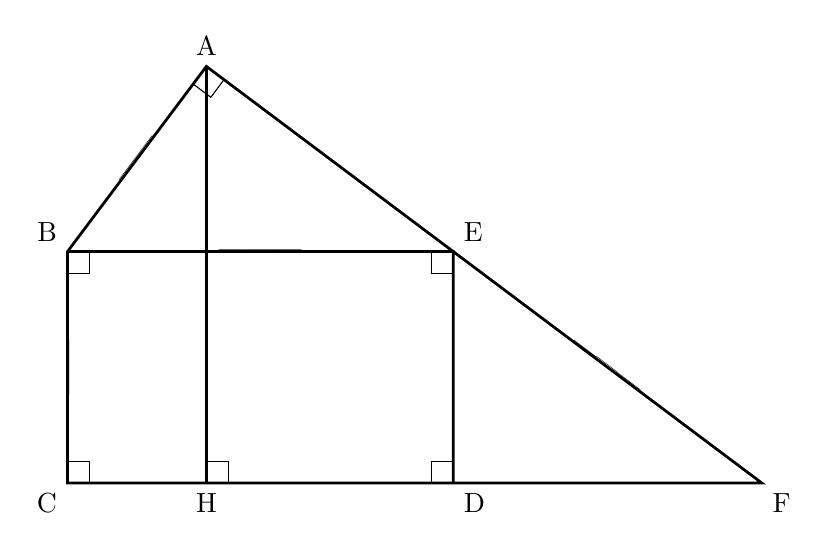
\begin{tikzpicture}[x=7mm,y=7mm]
	\draw[line width=1pt] (0,0) node[below left]{C}--
		(12.6,0.) node[below right] {F}--
		(2.52,7.56) node[pos = 0.28, sloped]{|||} node[above]{A}--
		(0.,4.2)node[pos = 0.5, sloped]{||} node[above left]{B} --cycle node[pos = 0.5, sloped]{||}
		(0.,4.2) -- (7.,4.2)node[pos = 0.5, sloped]{|||} node[above right]{E} -- (7.,0.) node[below right]{D}
		(2.52,0.) node[below] {H} -- (2.52,7.56);
		\foreach \x/\y in {0/0 , 2.52/0, 6.6/0, 6.6/3.8, 0/3.8}
			\draw[shift={(\x,\y)}] (0,0) rectangle (0.4,0.4) ;
		\draw[shift={(2.52,7.56)},rotate=143.13] (0,0) rectangle (-0.4,0.4) ;
\end{tikzpicture}
\end{center}

On donne :
\begin{itemize}[label={\textbullet~}]
	\item $\mathrm{AB}=\mathrm{BC}=4,2 \mathrm{~cm}$;
	\item $\mathrm{EB}=\mathrm{EF}=7 \mathrm{~cm}$.
\end{itemize}

\begin{enumerate}
	\item %Montrer que l'aire du rectangle BCDE est égale à \np[cm^2]{29,4}.
On a $\mathcal{A}(\text{BCDE}) = \text{BC} \times \text{EB} = 4,2 \times 7 = 29,4$~(cm$^2$).
	\item \begin{enumerate}
		\item Le théorème de Pythagore appliqué au triangle ABE, rectangle en A s'écrit :
		
$\text{BE}^2 = \text{AB}^2 + \text{AE}^2$, d'où $\text{AE}^2 = \text{BE}^2 - \text{AB}^2 = 7^2 - 4,2^2 = 49 - 17,64 = 31,36$. On a donc AE $= \sqrt{31,36} = 5,6$~(cm).
		
\emph{Rem.} $7^2 - 4,2^2 = (7 + 4,2)(7 - 4,2) = 11,2 \times 2,8 = 4  \times 2,8 \times 2,8 = 2^2 \times 2,8^2 = (2 \times 2,8)^2 = 5,6^2$. Donc AE est égale à \np[cm]{5,6}.
		
%Montrer que la longueur AE est égale à \np[cm]{5,6}.
		\item %Calculer l'aire du triangle rectangle ABE.
On a $\mathcal{A}(\text{ABE}) = \dfrac{\text{AB} \times \text{AE}}{2} = \dfrac{4,2 \times 5,6}{2} = 2,1 \times 5,6 = 11,76$~(cm$^2$).
	\end{enumerate}
	\item \begin{enumerate}
		\item %Montrer que les droites (ED) et (HA) sont parallèles.
Les droites (AH) et (ED) sont perpendiculaires à (FH) selon le codage, or lorsque deux droites sont perpendiculaires à une même droite, elles sont parallèles entre elles, on en conclut que (AH) et (ED) sont parallèles.
		\item %Calculer la longueur AH.
Les droites (AE) et (HD) sont sécantes en F et les droites (HA) et (ED) sont parallèles, donc d'après le théorème de Thalès :

$\dfrac{\text{FE}}{\text{FA}} = \dfrac{\text{FD}}{\text{FH}} = \dfrac{\text{ED}}{\text{AH}}$.

Comme FA = FE + EA $= 7 + 5,6 = 12,6$, on a en particulier :

$\dfrac{7}{2,6} = \dfrac{4,2}{\text{AH}}$ ; on en déduit que $7 \text{AH} = 4,2 \times 12,6$ et enfin 

$\text{AH} = \dfrac{4,2 \times 12,6}{7} = 0,6 \times 12,6 = 7,56$~(cm).

	\end{enumerate}
\end{enumerate}

\vspace{5mm}
%%%%%%%%

